A lógica computacional constitui um dos elementos fundamentais do desenvolvimento de software, estando relacionada à definição de regras, decisões, condições, operações e fluxos que determinam o comportamento de um sistema. A construção de um programa envolve, portanto, a organização desses elementos de maneira que possam ser interpretados e executados por um sistema computacional. Entretanto, a compreensão de um programa não depende exclusivamente da forma concreta em que suas instruções são escritas, uma vez que os elementos lógicos podem ser analisados em diferentes níveis de abstração.

A abstração constitui um mecanismo fundamental para lidar com a complexidade presente na computação. Por meio dela, características específicas de uma implementação podem ser ocultadas para que sejam considerados os elementos relevantes de um determinado problema. \citeonline{abelson1996} apresentam a abstração como um mecanismo importante para organizar sistemas computacionais e trabalhar com diferentes níveis de representação. Dessa forma, uma mesma estrutura computacional pode ser analisada considerando seus elementos fundamentais sem que seja necessário restringir sua compreensão a uma implementação específica. Essa perspectiva permite distinguir a lógica de um programa da forma utilizada para expressá-la.

A partir dessa possibilidade de abstração, diferentes formas de programação e representação foram desenvolvidas ao longo da evolução da computação. As linguagens de programação textuais expressam estruturas computacionais por meio de instruções e elementos sintáticos, enquanto abordagens visuais utilizam elementos gráficos para organizar e construir programas. Entre essas abordagens encontram-se linguagens baseadas em blocos, sistemas baseados em nós e outras formas de programação visual. \citeonline{myers1990} apresenta uma taxonomia das linguagens de programação visual, discutindo diferentes formas de utilizar representações gráficas como parte do processo de programação. O autor também diferencia programação visual de técnicas destinadas apenas à visualização de programas, distinção importante para esta pesquisa.

A programação visual, portanto, não deve ser compreendida simplesmente como uma representação gráfica de um código textual já existente. Em determinadas abordagens, os próprios elementos visuais constituem os mecanismos utilizados para construir a lógica do programa. Blocos, nós, conexões e outros componentes gráficos podem representar operações, relações, condições e fluxos, permitindo que o programa seja construído por meio dessas estruturas. Essa característica faz com que diferentes ambientes visuais possam apresentar formas distintas de organizar uma mesma classe de elementos computacionais.

A relação entre programação visual e programação textual também é discutida na literatura sob diferentes perspectivas. \citeonline{noone2018} realizaram uma revisão sistemática da literatura sobre linguagens de programação visuais e textuais, investigando principalmente seu papel no processo de aprendizagem de programação. A revisão reúne estudos que discutem as características e o uso dessas duas formas de programação, evidenciando que a relação entre representações visuais e textuais constitui um tema de investigação dentro da área de ensino de programação.

Além da revisão da literatura, existem estudos empíricos que analisam a utilização de ambientes visuais em situações concretas de aprendizagem. \citeonline{saezlopez2016} realizaram um estudo de dois anos em cinco escolas, envolvendo 107 estudantes, utilizando o Scratch como ambiente de programação visual. Por meio de uma abordagem quase-experimental, os autores observaram resultados relacionados à aprendizagem de conceitos de programação, lógica e práticas computacionais. Esses resultados fornecem evidência empírica sobre o uso de programação visual em um contexto educacional específico, mas não permitem afirmar que a programação visual seja universalmente superior à programação textual.

A combinação dessas perspectivas permite observar que a programação visual pode ser analisada tanto conceitualmente quanto empiricamente. \citeonline{myers1990} fornece uma base para compreender o que caracteriza uma representação visual utilizada na programação; \citeonline{noone2018} apresentam uma visão sistematizada da literatura sobre linguagens visuais e textuais; e \citeonline{saezlopez2016} apresentam evidências obtidas a partir da aplicação de um ambiente visual em um contexto educacional. Essas diferentes abordagens são relevantes para compreender que as formas de programação podem utilizar mecanismos de representação distintos, ainda que trabalhem com conceitos computacionais relacionados.

Nesse contexto, uma mesma estrutura lógica pode assumir diferentes formas de expressão. Uma condição, por exemplo, pode ser escrita por meio de uma estrutura textual, organizada por blocos ou representada por nós conectados em um fluxo. A alteração da representação não implica necessariamente uma alteração no comportamento lógico pretendido. Para esta pesquisa, essa distinção é fundamental, pois permite analisar separadamente a estrutura lógica de um programa e a forma utilizada para expressá-la.

Dessa perspectiva, este trabalho estabelece uma distinção entre lógica computacional e representação computacional. A lógica computacional corresponde ao conjunto de regras, operações, decisões e relações que determinam determinado comportamento, enquanto a representação computacional corresponde ao mecanismo utilizado para expressar esses elementos. Código textual, blocos e grafos de nós podem, portanto, constituir diferentes formas de representação de estruturas lógicas computacionais.

Entre as diferentes formas de programação visual, os sistemas baseados em nós constituem um caso particularmente relevante para esta investigação. Nesses ambientes, elementos gráficos são conectados para representar operações, eventos, condições e fluxos de execução. Um exemplo é o sistema de \textit{Blueprint Visual Scripting} da Unreal Engine, descrito por \citeonline{romero2014blueprint} como uma linguagem visual de programação baseada em nós. Nesse contexto, os \textit{Blueprints} constituem um exemplo concreto de como estruturas lógicas podem ser representadas visualmente e executadas em um ambiente computacional.

A existência de diferentes representações conduz a uma questão relacionada à comunicação e transformação entre essas formas. Quando uma lógica construída em uma determinada representação precisa ser expressa em outra, não basta necessariamente reproduzir seus elementos visuais ou sintáticos. É necessário identificar as estruturas e relações que determinam seu comportamento e preservá-las durante a transformação. Surge, assim, o problema de investigar como diferentes representações podem estabelecer correspondências entre si sem perder os elementos fundamentais da lógica computacional.

Nesse cenário, a Inteligência Artificial apresenta uma possibilidade de apoio à interpretação e transformação dessas representações. Modelos capazes de processar linguagem e estruturas de código podem receber uma representação de origem, interpretar seus elementos e produzir uma representação em outro formato. Entretanto, é necessário investigar em que medida esses modelos conseguem preservar a lógica presente na representação original e quais mecanismos podem contribuir para essa preservação.

Uma possibilidade considerada neste trabalho é a utilização de uma representação lógica intermediária, capaz de organizar os elementos comuns entre diferentes formas de programação. Essa estrutura poderia funcionar como uma camada de correspondência entre uma representação de origem e uma representação de destino, permitindo que a transformação não dependa exclusivamente de uma relação direta entre dois formatos específicos. Essa possibilidade constitui uma hipótese da pesquisa e será investigada experimentalmente.

A partir dessa problemática, este trabalho investiga como a Inteligência Artificial pode auxiliar na transformação entre diferentes representações da lógica computacional, com ênfase na relação entre representações textuais e visuais. Parte-se da hipótese de que uma representação lógica intermediária pode auxiliar na identificação e preservação dos elementos fundamentais de uma lógica durante sua transformação entre diferentes formas de representação.

Como objetivo geral, pretende-se investigar como técnicas de Inteligência Artificial podem auxiliar na transformação entre representações visuais e textuais da lógica computacional, analisando a preservação dos elementos lógicos envolvidos nesse processo. Como objetivos específicos, busca-se identificar características das representações visuais e textuais utilizadas para expressar lógica computacional; analisar diferentes formas de programação visual; identificar correspondências entre elementos presentes nas representações analisadas; investigar a utilização de modelos de Inteligência Artificial na transformação entre representações; e avaliar os resultados dessas transformações considerando a preservação da lógica computacional.

Do ponto de vista metodológico, esta pesquisa caracteriza-se como básica, de natureza qualitativa e de objetivos exploratórios \cite{gil2002}. Inicialmente, será realizada pesquisa bibliográfica sobre lógica computacional, abstração, representação, programação visual, programação textual e Inteligência Artificial. Também será realizada pesquisa documental \cite{prodanov2013}, considerando diferentes ambientes e exemplos de programação visual e textual. Posteriormente, serão realizados experimentos controlados com modelos de Inteligência Artificial para investigar a transformação entre representações e avaliar a preservação da lógica computacional nas saídas produzidas.

A Figura~\ref{fig:figura1_traducao_representacoes} apresenta, de forma conceitual, a relação investigada neste trabalho entre diferentes formas de representação da lógica computacional e o processo de transformação assistido por Inteligência Artificial.

\begin{figure}[H]
    \centering
    \caption{Representação conceitual da transformação entre representações visuais e textuais da lógica computacional.}
    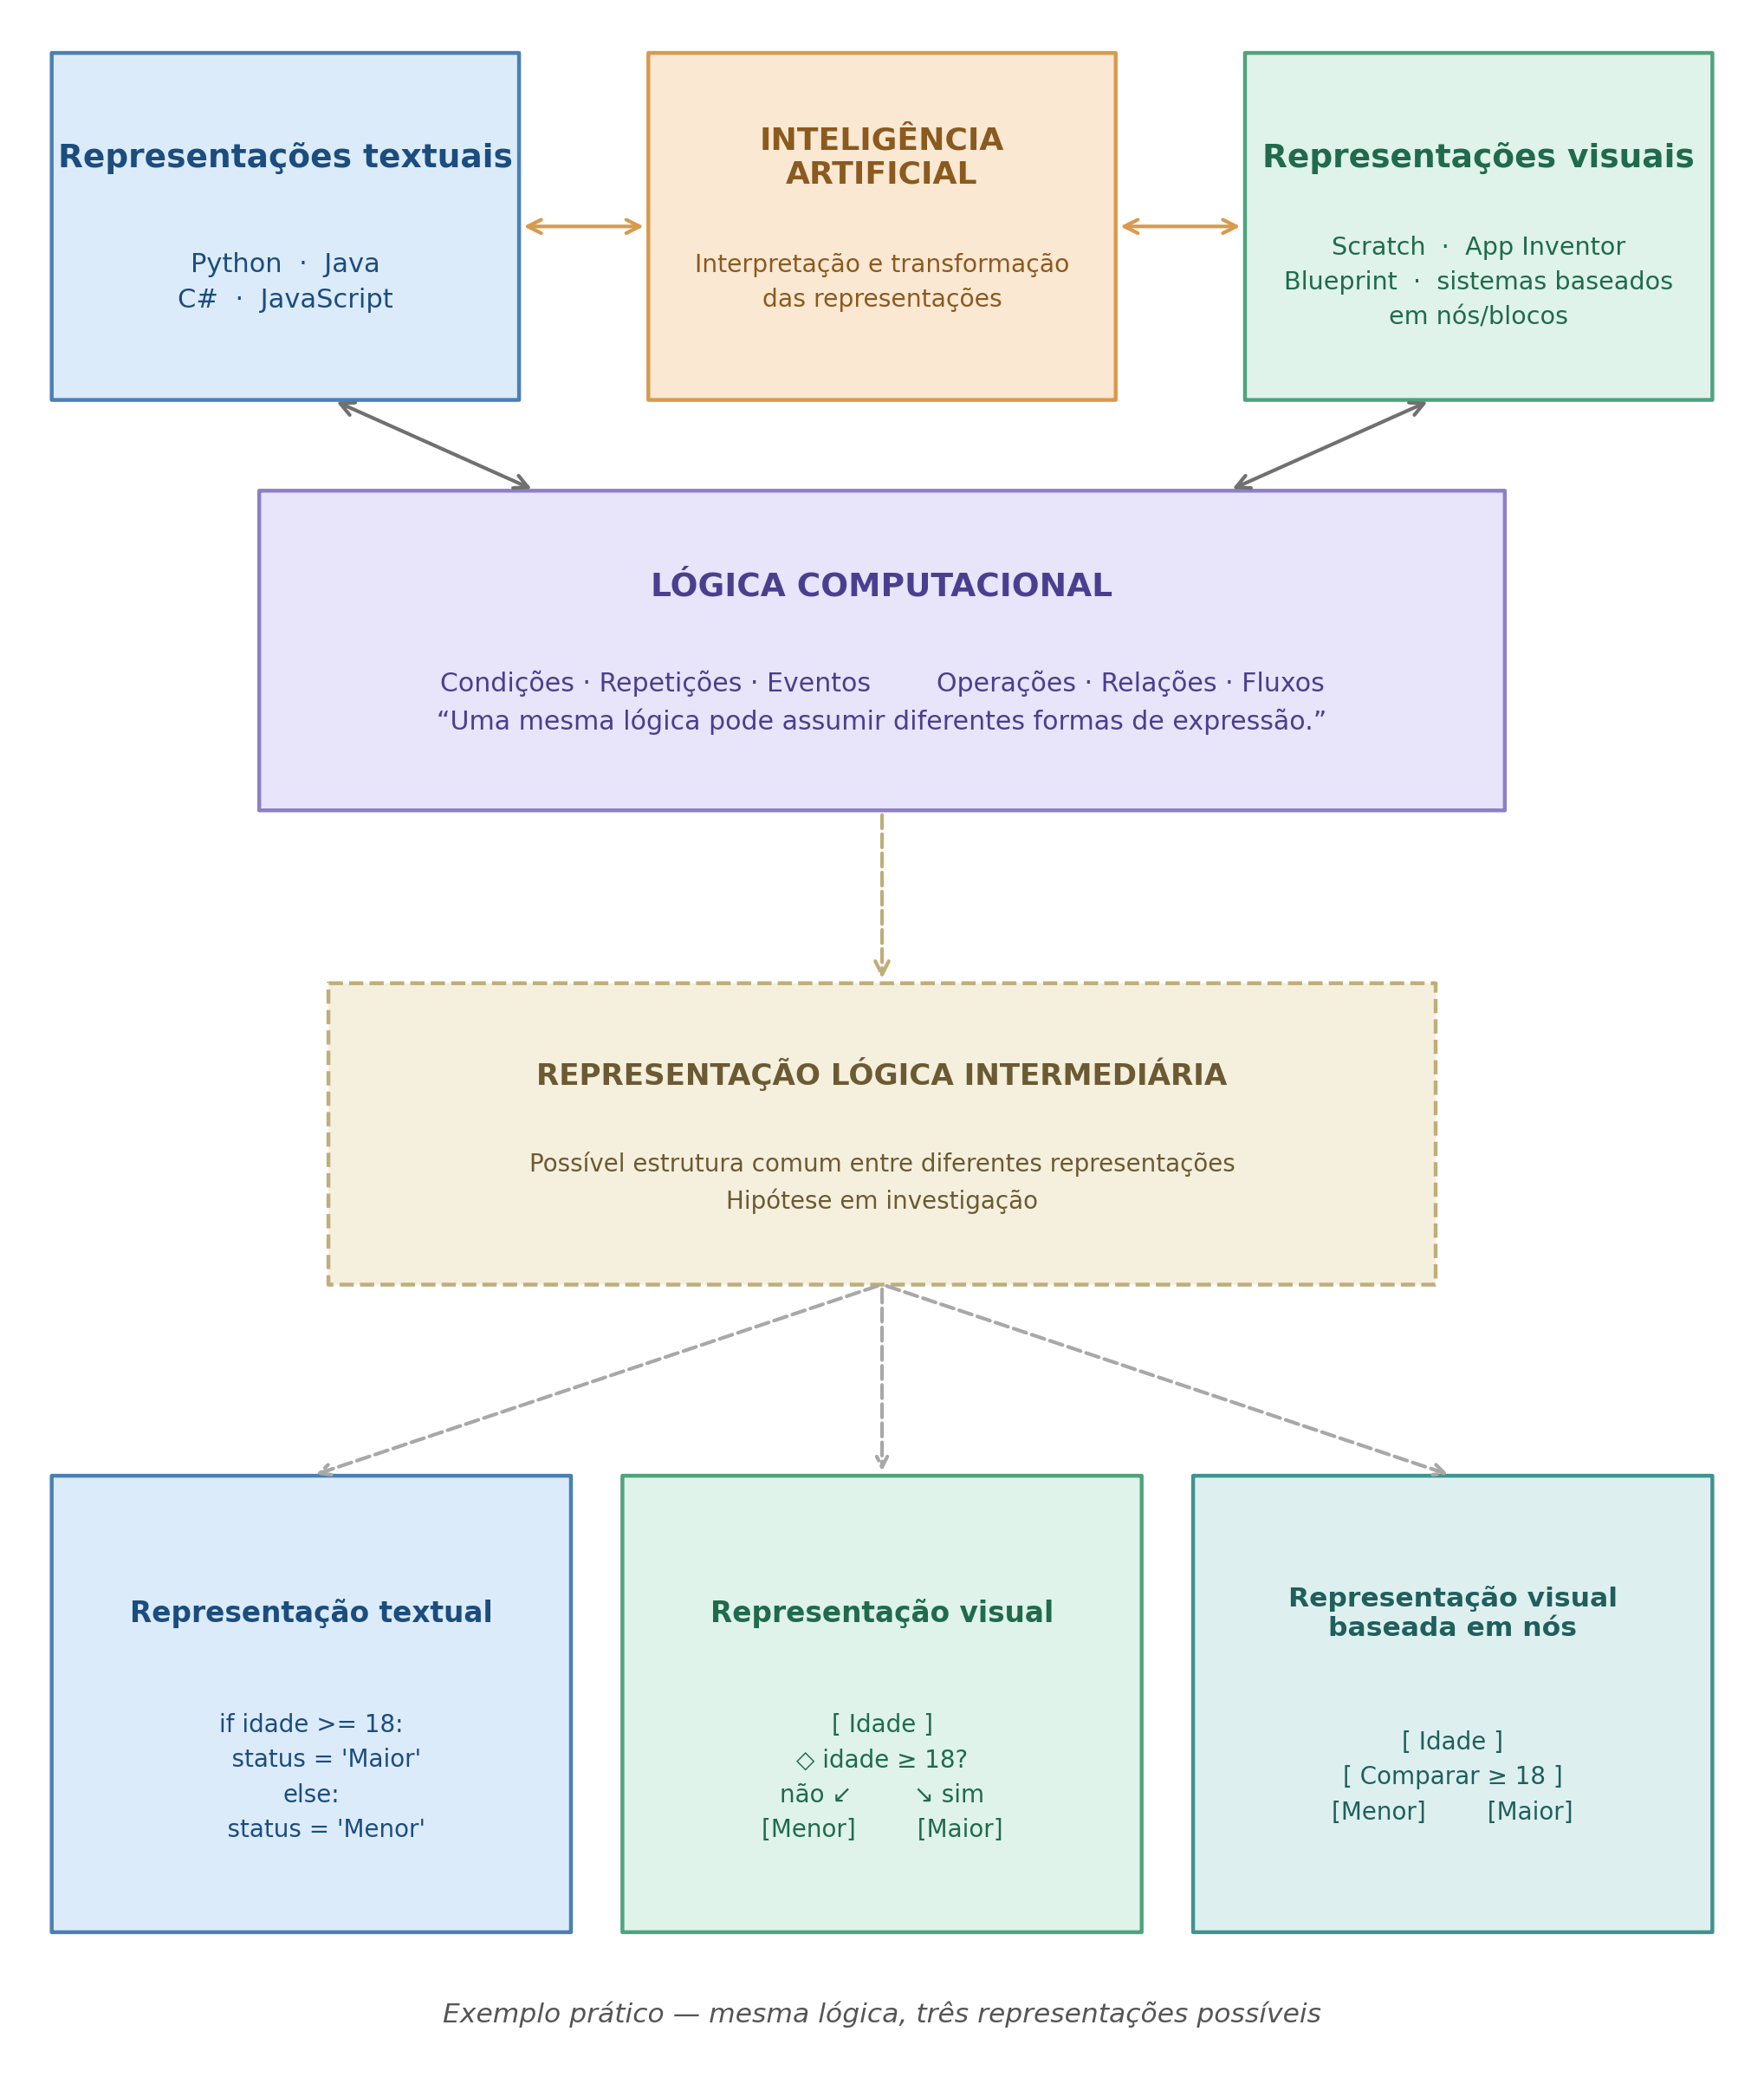
\includegraphics[width=\textwidth]{images/figura1_traducao_representacoes.png}
    \legend{Fonte: elaboração do autor com base em \citeonline{abelson1996} e \citeonline{myers1990}.}
    \label{fig:figura1_traducao_representacoes}
\end{figure}